\section{Benchmark NIST-11 "Intersecting Interfaces"}
\label{sec:bench-11}

The solution to this elliptic problems contains a severe
singularity that poses a challenge to adaptive methods.
The equation is given as below

\begin{equation} \label{intersecting}
-\nabla \cdot (a(x,y) \nabla u) = 0
\end{equation}
where the parameter $a$ is piecewise-constant,
$a(x,y) = R$ in the first and third quadrants
and $a(x,y) = 1$ in the remaining two quadrants.
The domain of this problem is $\Omega = (-1, 1)^2$, equipped with
Dirichlet boundary conditions given by the exact solution.

The exact solution
\begin{equation}\label{exact-nist-11}
u(x,y) = r^{a} \mu
\end{equation}

The solution of NIST-11 is shown in Fig. \ref{fig:sln-nist11}.

\begin{figure}[!ht]
\centering
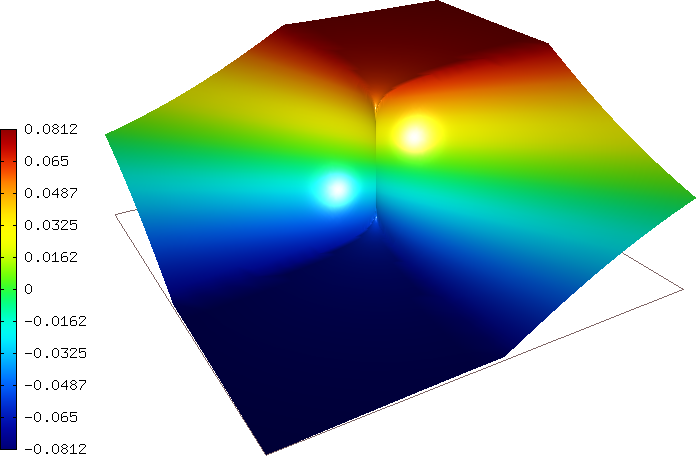
\includegraphics[height=6cm]{nist/nist-11/solution.png}
\caption{The solution to NIST-11 benchmark problem.}
\label{fig:sln-nist11}
\end{figure}
